\item An object of mass ‘m’ initially at rest on a smooth horizontal plane starts moving under the action of force F = 2N. In the process of its linear motion. The angle $\theta$ (as shown in figure) between the direction of force and horizontal varies as $\theta = kx$, where $k$ is a constant and $x$ is the distance covered by the object from its initial position. The expression of kinetic energy of the object will be $E = \frac{n}{k} \sin \theta$. The value of $n$ is \underline{\hspace{2.5cm}}.
    \begin{center}
        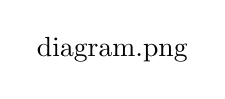
\begin{tikzpicture}
            \node at (0, 0) {{diagram.png}};
        \end{tikzpicture}
    \end{center}